\documentclass[aspectratio=169]{beamer}
\usetheme{Bruno}
\usepackage{amsmath}
\usepackage{amssymb}
\usepackage{siunitx}
\usepackage{float}
\usepackage{tikz}
\usetikzlibrary{circuits.plc.ladder}
\usepackage{tikz-cd}
\usepackage{url}
\usepackage[siunitx,american,RPvoltages]{circuitikz}
\ctikzset{capacitors/scale=0.7}
\ctikzset{diodes/scale=0.7}
\usepackage{tabularx}
\newcolumntype{C}{>{\centering\arraybackslash}X}
\renewcommand\tabularxcolumn[1]{m{#1}}% for vertical centering text in X column
\usepackage{tabu}
\usepackage[spanish,es-tabla,activeacute]{babel}
\usepackage{babelbib}
\usepackage{booktabs}
\usepackage{pgfplots}
\usepackage{hyperref}
\hypersetup{colorlinks = true,
            linkcolor = black,
            urlcolor  = blue,
            citecolor = blue,
            anchorcolor = blue}
\usepgfplotslibrary{units, fillbetween} 
\pgfplotsset{compat=1.16}
\usepackage{bm}
\usetikzlibrary{arrows, arrows.meta, shapes, 3d, perspective, positioning}
\renewcommand{\sin}{\sen} %change from sin to sen
\usepackage{bohr}
\setbohr{distribution-method = quantum,insert-missing = true}
\usepackage{elements}
\usepackage{verbatim}
\usetikzlibrary{mindmap,trees,backgrounds}
\definecolor{color_mate}{RGB}{255,255,128}
\definecolor{color_plas}{RGB}{255,128,255}
\definecolor{color_text}{RGB}{128,255,255}
\definecolor{color_petr}{RGB}{255,192,192}
\definecolor{color_made}{RGB}{192,255,192}
\definecolor{color_meta}{RGB}{192,192,255}
\usepackage[edges]{forest}
\usepackage{etoolbox}
\usepackage{schemata}
\newcommand\diagram[2]{\schema{\schemabox{#1}}{\schemabox{#2}}}
\usepackage{listings}
\usepackage{csvsimple}
 %%%%%%%%%%%%%%%%%%%%%%%%%%%%%%%%%%%%%%%%%%%%%%%%%%%%%%%%%%%%%%%%%%%%%%%%%%%%%%%% 
%%% ~ Arduino Language - Arduino IDE Colors ~                                  %%%
%%%                                                                            %%%
%%% Kyle Rocha-Brownell | 10/2/2017 | No Licence                               %%%
%%% -------------------------------------------------------------------------- %%%
%%%                                                                            %%%
%%% Place this file in your working directory (next to the latex file you're   %%%
%%% working on).  To add it to your project, place:                            %%%
%%%     %%%%%%%%%%%%%%%%%%%%%%%%%%%%%%%%%%%%%%%%%%%%%%%%%%%%%%%%%%%%%%%%%%%%%%%%%%%%%%%% 
%%% ~ Arduino Language - Arduino IDE Colors ~                                  %%%
%%%                                                                            %%%
%%% Kyle Rocha-Brownell | 10/2/2017 | No Licence                               %%%
%%% -------------------------------------------------------------------------- %%%
%%%                                                                            %%%
%%% Place this file in your working directory (next to the latex file you're   %%%
%%% working on).  To add it to your project, place:                            %%%
%%%    \input{arduinoLanguage.tex}                                             %%%
%%% somewhere before \begin{document} in your latex file.                      %%%
%%%                                                                            %%%
%%% In your document, place your arduino code between:                         %%%
%%%   \begin{lstlisting}[language=Arduino]                                     %%%
%%% and:                                                                       %%%
%%%   \end{lstlisting}                                                         %%%
%%%                                                                            %%%
%%% Or create your own style to add non-built-in functions and variables.      %%%
%%%                                                                            %%%
 %%%%%%%%%%%%%%%%%%%%%%%%%%%%%%%%%%%%%%%%%%%%%%%%%%%%%%%%%%%%%%%%%%%%%%%%%%%%%%%% 

\usepackage{color}
\usepackage{listings}    
\usepackage{courier}

%%% Define Custom IDE Colors %%%
\definecolor{arduinoGreen}    {rgb} {0.17, 0.43, 0.01}
\definecolor{arduinoGrey}     {rgb} {0.47, 0.47, 0.33}
\definecolor{arduinoOrange}   {rgb} {0.8 , 0.4 , 0   }
\definecolor{arduinoBlue}     {rgb} {0.01, 0.61, 0.98}
\definecolor{arduinoDarkBlue} {rgb} {0.0 , 0.2 , 0.5 }

%%% Define Arduino Language %%%
\lstdefinelanguage{Arduino}{
  language=C++, % begin with default C++ settings 
%
%
  %%% Keyword Color Group 1 %%%  (called KEYWORD3 by arduino)
  keywordstyle=\color{arduinoGreen},   
  deletekeywords={  % remove all arduino keywords that might be in c++
                break, case, override, final, continue, default, do, else, for, 
                if, return, goto, switch, throw, try, while, setup, loop, export, 
                not, or, and, xor, include, define, elif, else, error, if, ifdef, 
                ifndef, pragma, warning,
                HIGH, LOW, INPUT, INPUT_PULLUP, OUTPUT, DEC, BIN, HEX, OCT, PI, 
                HALF_PI, TWO_PI, LSBFIRST, MSBFIRST, CHANGE, FALLING, RISING, 
                DEFAULT, EXTERNAL, INTERNAL, INTERNAL1V1, INTERNAL2V56, LED_BUILTIN, 
                LED_BUILTIN_RX, LED_BUILTIN_TX, DIGITAL_MESSAGE, FIRMATA_STRING, 
                ANALOG_MESSAGE, REPORT_DIGITAL, REPORT_ANALOG, SET_PIN_MODE, 
                SYSTEM_RESET, SYSEX_START, auto, int8_t, int16_t, int32_t, int64_t, 
                uint8_t, uint16_t, uint32_t, uint64_t, char16_t, char32_t, operator, 
                enum, delete, bool, boolean, byte, char, const, false, float, double, 
                null, NULL, int, long, new, private, protected, public, short, 
                signed, static, volatile, String, void, true, unsigned, word, array, 
                sizeof, dynamic_cast, typedef, const_cast, struct, static_cast, union, 
                friend, extern, class, reinterpret_cast, register, explicit, inline, 
                _Bool, complex, _Complex, _Imaginary, atomic_bool, atomic_char, 
                atomic_schar, atomic_uchar, atomic_short, atomic_ushort, atomic_int, 
                atomic_uint, atomic_long, atomic_ulong, atomic_llong, atomic_ullong, 
                virtual, PROGMEM,
                Serial, Serial1, Serial2, Serial3, SerialUSB, Keyboard, Mouse,
                abs, acos, asin, atan, atan2, ceil, constrain, cos, degrees, exp, 
                floor, log, map, max, min, radians, random, randomSeed, round, sin, 
                sq, sqrt, tan, pow, bitRead, bitWrite, bitSet, bitClear, bit, 
                highByte, lowByte, analogReference, analogRead, 
                analogReadResolution, analogWrite, analogWriteResolution, 
                attachInterrupt, detachInterrupt, digitalPinToInterrupt, delay, 
                delayMicroseconds, digitalWrite, digitalRead, interrupts, millis, 
                micros, noInterrupts, noTone, pinMode, pulseIn, pulseInLong, shiftIn, 
                shiftOut, tone, yield, Stream, begin, end, peek, read, print, 
                println, available, availableForWrite, flush, setTimeout, find, 
                findUntil, parseInt, parseFloat, readBytes, readBytesUntil, readString, 
                readStringUntil, trim, toUpperCase, toLowerCase, charAt, compareTo, 
                concat, endsWith, startsWith, equals, equalsIgnoreCase, getBytes, 
                indexOf, lastIndexOf, length, replace, setCharAt, substring, 
                toCharArray, toInt, press, release, releaseAll, accept, click, move, 
                isPressed, isAlphaNumeric, isAlpha, isAscii, isWhitespace, isControl, 
                isDigit, isGraph, isLowerCase, isPrintable, isPunct, isSpace, 
                isUpperCase, isHexadecimalDigit, 
                }, 
  morekeywords={   % add arduino structures to group 1
                break, case, override, final, continue, default, do, else, for, 
                if, return, goto, switch, throw, try, while, setup, loop, export, 
                not, or, and, xor, include, define, elif, else, error, if, ifdef, 
                ifndef, pragma, warning,
                }, 
% 
%
  %%% Keyword Color Group 2 %%%  (called LITERAL1 by arduino)
  keywordstyle=[2]\color{arduinoBlue},   
  keywords=[2]{   % add variables and dataTypes as 2nd group  
                HIGH, LOW, INPUT, INPUT_PULLUP, OUTPUT, DEC, BIN, HEX, OCT, PI, 
                HALF_PI, TWO_PI, LSBFIRST, MSBFIRST, CHANGE, FALLING, RISING, 
                DEFAULT, EXTERNAL, INTERNAL, INTERNAL1V1, INTERNAL2V56, LED_BUILTIN, 
                LED_BUILTIN_RX, LED_BUILTIN_TX, DIGITAL_MESSAGE, FIRMATA_STRING, 
                ANALOG_MESSAGE, REPORT_DIGITAL, REPORT_ANALOG, SET_PIN_MODE, 
                SYSTEM_RESET, SYSEX_START, auto, int8_t, int16_t, int32_t, int64_t, 
                uint8_t, uint16_t, uint32_t, uint64_t, char16_t, char32_t, operator, 
                enum, delete, bool, boolean, byte, char, const, false, float, double, 
                null, NULL, int, long, new, private, protected, public, short, 
                signed, static, volatile, String, void, true, unsigned, word, array, 
                sizeof, dynamic_cast, typedef, const_cast, struct, static_cast, union, 
                friend, extern, class, reinterpret_cast, register, explicit, inline, 
                _Bool, complex, _Complex, _Imaginary, atomic_bool, atomic_char, 
                atomic_schar, atomic_uchar, atomic_short, atomic_ushort, atomic_int, 
                atomic_uint, atomic_long, atomic_ulong, atomic_llong, atomic_ullong, 
                virtual, PROGMEM,
                },  
% 
%
  %%% Keyword Color Group 3 %%%  (called KEYWORD1 by arduino)
  keywordstyle=[3]\bfseries\color{arduinoOrange},
  keywords=[3]{  % add built-in functions as a 3rd group
                Serial, Serial1, Serial2, Serial3, SerialUSB, Keyboard, Mouse,
                },      
%
%
  %%% Keyword Color Group 4 %%%  (called KEYWORD2 by arduino)
  keywordstyle=[4]\color{arduinoOrange},
  keywords=[4]{  % add more built-in functions as a 4th group
                abs, acos, asin, atan, atan2, ceil, constrain, cos, degrees, exp, 
                floor, log, map, max, min, radians, random, randomSeed, round, sin, 
                sq, sqrt, tan, pow, bitRead, bitWrite, bitSet, bitClear, bit, 
                highByte, lowByte, analogReference, analogRead, 
                analogReadResolution, analogWrite, analogWriteResolution, 
                attachInterrupt, detachInterrupt, digitalPinToInterrupt, delay, 
                delayMicroseconds, digitalWrite, digitalRead, interrupts, millis, 
                micros, noInterrupts, noTone, pinMode, pulseIn, pulseInLong, shiftIn, 
                shiftOut, tone, yield, Stream, begin, end, peek, read, print, 
                println, available, availableForWrite, flush, setTimeout, find, 
                findUntil, parseInt, parseFloat, readBytes, readBytesUntil, readString, 
                readStringUntil, trim, toUpperCase, toLowerCase, charAt, compareTo, 
                concat, endsWith, startsWith, equals, equalsIgnoreCase, getBytes, 
                indexOf, lastIndexOf, length, replace, setCharAt, substring, 
                toCharArray, toInt, press, release, releaseAll, accept, click, move, 
                isPressed, isAlphaNumeric, isAlpha, isAscii, isWhitespace, isControl, 
                isDigit, isGraph, isLowerCase, isPrintable, isPunct, isSpace, 
                isUpperCase, isHexadecimalDigit, 
                },      
%
%
  %%% Set Other Colors %%%
  stringstyle=\color{arduinoDarkBlue},    
  commentstyle=\color{arduinoGrey},    
%          
%   
  %%%% Line Numbering %%%%
   numbers=left,                    
  numbersep=5pt,                   
  numberstyle=\color{arduinoGrey},    
  %stepnumber=2,                      % show every 2 line numbers
%
%
  %%%% Code Box Style %%%%
  breaklines=true,                    % wordwrapping
  tabsize=2,         
  basicstyle=\ttfamily  
}                                             %%%
%%% somewhere before \begin{document} in your latex file.                      %%%
%%%                                                                            %%%
%%% In your document, place your arduino code between:                         %%%
%%%   \begin{lstlisting}[language=Arduino]                                     %%%
%%% and:                                                                       %%%
%%%   \end{lstlisting}                                                         %%%
%%%                                                                            %%%
%%% Or create your own style to add non-built-in functions and variables.      %%%
%%%                                                                            %%%
 %%%%%%%%%%%%%%%%%%%%%%%%%%%%%%%%%%%%%%%%%%%%%%%%%%%%%%%%%%%%%%%%%%%%%%%%%%%%%%%% 

\usepackage{color}
\usepackage{listings}    
\usepackage{courier}

%%% Define Custom IDE Colors %%%
\definecolor{arduinoGreen}    {rgb} {0.17, 0.43, 0.01}
\definecolor{arduinoGrey}     {rgb} {0.47, 0.47, 0.33}
\definecolor{arduinoOrange}   {rgb} {0.8 , 0.4 , 0   }
\definecolor{arduinoBlue}     {rgb} {0.01, 0.61, 0.98}
\definecolor{arduinoDarkBlue} {rgb} {0.0 , 0.2 , 0.5 }

%%% Define Arduino Language %%%
\lstdefinelanguage{Arduino}{
  language=C++, % begin with default C++ settings 
%
%
  %%% Keyword Color Group 1 %%%  (called KEYWORD3 by arduino)
  keywordstyle=\color{arduinoGreen},   
  deletekeywords={  % remove all arduino keywords that might be in c++
                break, case, override, final, continue, default, do, else, for, 
                if, return, goto, switch, throw, try, while, setup, loop, export, 
                not, or, and, xor, include, define, elif, else, error, if, ifdef, 
                ifndef, pragma, warning,
                HIGH, LOW, INPUT, INPUT_PULLUP, OUTPUT, DEC, BIN, HEX, OCT, PI, 
                HALF_PI, TWO_PI, LSBFIRST, MSBFIRST, CHANGE, FALLING, RISING, 
                DEFAULT, EXTERNAL, INTERNAL, INTERNAL1V1, INTERNAL2V56, LED_BUILTIN, 
                LED_BUILTIN_RX, LED_BUILTIN_TX, DIGITAL_MESSAGE, FIRMATA_STRING, 
                ANALOG_MESSAGE, REPORT_DIGITAL, REPORT_ANALOG, SET_PIN_MODE, 
                SYSTEM_RESET, SYSEX_START, auto, int8_t, int16_t, int32_t, int64_t, 
                uint8_t, uint16_t, uint32_t, uint64_t, char16_t, char32_t, operator, 
                enum, delete, bool, boolean, byte, char, const, false, float, double, 
                null, NULL, int, long, new, private, protected, public, short, 
                signed, static, volatile, String, void, true, unsigned, word, array, 
                sizeof, dynamic_cast, typedef, const_cast, struct, static_cast, union, 
                friend, extern, class, reinterpret_cast, register, explicit, inline, 
                _Bool, complex, _Complex, _Imaginary, atomic_bool, atomic_char, 
                atomic_schar, atomic_uchar, atomic_short, atomic_ushort, atomic_int, 
                atomic_uint, atomic_long, atomic_ulong, atomic_llong, atomic_ullong, 
                virtual, PROGMEM,
                Serial, Serial1, Serial2, Serial3, SerialUSB, Keyboard, Mouse,
                abs, acos, asin, atan, atan2, ceil, constrain, cos, degrees, exp, 
                floor, log, map, max, min, radians, random, randomSeed, round, sin, 
                sq, sqrt, tan, pow, bitRead, bitWrite, bitSet, bitClear, bit, 
                highByte, lowByte, analogReference, analogRead, 
                analogReadResolution, analogWrite, analogWriteResolution, 
                attachInterrupt, detachInterrupt, digitalPinToInterrupt, delay, 
                delayMicroseconds, digitalWrite, digitalRead, interrupts, millis, 
                micros, noInterrupts, noTone, pinMode, pulseIn, pulseInLong, shiftIn, 
                shiftOut, tone, yield, Stream, begin, end, peek, read, print, 
                println, available, availableForWrite, flush, setTimeout, find, 
                findUntil, parseInt, parseFloat, readBytes, readBytesUntil, readString, 
                readStringUntil, trim, toUpperCase, toLowerCase, charAt, compareTo, 
                concat, endsWith, startsWith, equals, equalsIgnoreCase, getBytes, 
                indexOf, lastIndexOf, length, replace, setCharAt, substring, 
                toCharArray, toInt, press, release, releaseAll, accept, click, move, 
                isPressed, isAlphaNumeric, isAlpha, isAscii, isWhitespace, isControl, 
                isDigit, isGraph, isLowerCase, isPrintable, isPunct, isSpace, 
                isUpperCase, isHexadecimalDigit, 
                }, 
  morekeywords={   % add arduino structures to group 1
                break, case, override, final, continue, default, do, else, for, 
                if, return, goto, switch, throw, try, while, setup, loop, export, 
                not, or, and, xor, include, define, elif, else, error, if, ifdef, 
                ifndef, pragma, warning,
                }, 
% 
%
  %%% Keyword Color Group 2 %%%  (called LITERAL1 by arduino)
  keywordstyle=[2]\color{arduinoBlue},   
  keywords=[2]{   % add variables and dataTypes as 2nd group  
                HIGH, LOW, INPUT, INPUT_PULLUP, OUTPUT, DEC, BIN, HEX, OCT, PI, 
                HALF_PI, TWO_PI, LSBFIRST, MSBFIRST, CHANGE, FALLING, RISING, 
                DEFAULT, EXTERNAL, INTERNAL, INTERNAL1V1, INTERNAL2V56, LED_BUILTIN, 
                LED_BUILTIN_RX, LED_BUILTIN_TX, DIGITAL_MESSAGE, FIRMATA_STRING, 
                ANALOG_MESSAGE, REPORT_DIGITAL, REPORT_ANALOG, SET_PIN_MODE, 
                SYSTEM_RESET, SYSEX_START, auto, int8_t, int16_t, int32_t, int64_t, 
                uint8_t, uint16_t, uint32_t, uint64_t, char16_t, char32_t, operator, 
                enum, delete, bool, boolean, byte, char, const, false, float, double, 
                null, NULL, int, long, new, private, protected, public, short, 
                signed, static, volatile, String, void, true, unsigned, word, array, 
                sizeof, dynamic_cast, typedef, const_cast, struct, static_cast, union, 
                friend, extern, class, reinterpret_cast, register, explicit, inline, 
                _Bool, complex, _Complex, _Imaginary, atomic_bool, atomic_char, 
                atomic_schar, atomic_uchar, atomic_short, atomic_ushort, atomic_int, 
                atomic_uint, atomic_long, atomic_ulong, atomic_llong, atomic_ullong, 
                virtual, PROGMEM,
                },  
% 
%
  %%% Keyword Color Group 3 %%%  (called KEYWORD1 by arduino)
  keywordstyle=[3]\bfseries\color{arduinoOrange},
  keywords=[3]{  % add built-in functions as a 3rd group
                Serial, Serial1, Serial2, Serial3, SerialUSB, Keyboard, Mouse,
                },      
%
%
  %%% Keyword Color Group 4 %%%  (called KEYWORD2 by arduino)
  keywordstyle=[4]\color{arduinoOrange},
  keywords=[4]{  % add more built-in functions as a 4th group
                abs, acos, asin, atan, atan2, ceil, constrain, cos, degrees, exp, 
                floor, log, map, max, min, radians, random, randomSeed, round, sin, 
                sq, sqrt, tan, pow, bitRead, bitWrite, bitSet, bitClear, bit, 
                highByte, lowByte, analogReference, analogRead, 
                analogReadResolution, analogWrite, analogWriteResolution, 
                attachInterrupt, detachInterrupt, digitalPinToInterrupt, delay, 
                delayMicroseconds, digitalWrite, digitalRead, interrupts, millis, 
                micros, noInterrupts, noTone, pinMode, pulseIn, pulseInLong, shiftIn, 
                shiftOut, tone, yield, Stream, begin, end, peek, read, print, 
                println, available, availableForWrite, flush, setTimeout, find, 
                findUntil, parseInt, parseFloat, readBytes, readBytesUntil, readString, 
                readStringUntil, trim, toUpperCase, toLowerCase, charAt, compareTo, 
                concat, endsWith, startsWith, equals, equalsIgnoreCase, getBytes, 
                indexOf, lastIndexOf, length, replace, setCharAt, substring, 
                toCharArray, toInt, press, release, releaseAll, accept, click, move, 
                isPressed, isAlphaNumeric, isAlpha, isAscii, isWhitespace, isControl, 
                isDigit, isGraph, isLowerCase, isPrintable, isPunct, isSpace, 
                isUpperCase, isHexadecimalDigit, 
                },      
%
%
  %%% Set Other Colors %%%
  stringstyle=\color{arduinoDarkBlue},    
  commentstyle=\color{arduinoGrey},    
%          
%   
  %%%% Line Numbering %%%%
   numbers=left,                    
  numbersep=5pt,                   
  numberstyle=\color{arduinoGrey},    
  %stepnumber=2,                      % show every 2 line numbers
%
%
  %%%% Code Box Style %%%%
  breaklines=true,                    % wordwrapping
  tabsize=2,         
  basicstyle=\ttfamily  
}
\usepackage{lmodern}
\usepackage{subcaption}

\graphicspath{{../fig/}}


\title{Instrumentación I: \\ \emph{Introducción a la }\\ \emph{instrumentación industrial.} \\ \emph{Segunda sesión}}
\author{
    Juan J. Rojas, Hugo Sanchez Ortiz
}
\institute{Instituto Tecnológico de Costa Rica}
\date{\today}
\background{fig/background.jpg}
\begin{document}
%\sisetup{unit-math-rm=\mathrm,math-rm=\mathrm} % change sinitx font
\sisetup{output-decimal-marker = {,}}
\maketitle

\newcommand{\blackandwhite}{white} %change this at the end

\begin{frame}{Rangos de entrada y sálida, sesgo de sensado}
    \begin{columns}[c, onlytextwidth]
        \begin{column}{0.50\textwidth}
            \begin{itemize}
                \item Rango del estímulo (span): representa la diferencia entre el valor mínimo y el valor máximo del estímulo que pueden medirse con un error aceptable.
                \item Salida a escala completa (full-scale output, FSO): representa la diferencia entre los valores de la señal de salida que corresponden al valor mínimo y máximo del estímulo medido. 
            \end{itemize}
        \end{column}
        \begin{column}{0.45\textwidth}
            \textbf{Ejemplo}\\[4pt]
            Marca: Amphenol\\[4pt]
            Modelo: NovaSensor NPI-19\\[4pt]
            Estímulo: presión\\[4pt]
            Tipo: piezoresistivo\\[4pt]
            Rango del estímulo: $0  - \SI{17.2}{\kilo\pascal}$\\[4pt]
            Salida a escala completa: $\SI{125}{\milli\volt}$\\[4pt]
            Sesgo de sensado: $\pm \SI{1}{\milli\volt}$\\[10pt]
            \tiny{Tomado de \href{https://f.hubspotusercontent40.net/hubfs/9035299/Product\%20Documents/AAS-920-298B-NovaSensor\%20NPI-19-REVISED-061714-web\%20(1).pdf}{aquí}}
        \end{column}
    \end{columns}
\end{frame}

\begin{frame}{Sesgo de sensado e histeresis}
    \begin{columns}[c, onlytextwidth]
        \begin{column}{0.50\textwidth}
            \begin{itemize}
                \item Sesgo de sensado (offset): es el rango de valores de la señal de salida cuando el estimulo tiene valor cero. 
                \item Histéresis: es una desviación de la señal de salida  que se obtiene al realizar la medición de un mismo valor de un estímulo en direcciones opuestas.
            \end{itemize}
        \end{column}
        \begin{column}{0.45\textwidth}
            \textbf{Ejemplo}\\[4pt]
            Marca: Allen-Bradley\\[4pt]
            Modelo: 875C AC\\[4pt]
            Estímulo: posición\\[4pt]
            Tipo: capacitivo\\[4pt]
            Histéresis: $\leq 10 \%$\\[10pt]
            \tiny{Tomado de \href{https://literature.rockwellautomation.com/idc/groups/literature/documents/td/875c-td001_-en-p.pdf}{aquí}}
        \end{column}
    \end{columns}
\end{frame}

\begin{frame}{Exactitud y precisión}
    \begin{columns}[c, onlytextwidth]
        \begin{column}{0.55\textwidth}
            \begin{itemize}
                \item Valor real de un estimulo: es el que se obtendría con una medición perfecta. Sin embargo este valor es indeterminado y por lo tanto se define por algún tipo de convención. 
                \item Exactitud: es la capacidad de un sensor de dar un resultado cercano al valor real del estímulo medido.
                \item Precisión: es la capacidad de un sensor de dar el mismo resultado cuando se mide el mismo valor de un estimulo bajo las mismas condiciones. 
            \end{itemize}
        \end{column}
        \begin{column}{0.40\textwidth}
            \textbf{Ejemplo}\\[4pt]
            Marca: Amphenol\\[4pt]
            Modelo: NovaSensor NPI-19\\[4pt]
            Estímulo: presión\\[4pt]
            Tipo: piezoresistivo\\[4pt]
            Exactitud estática$^*$: $0.1 \%$ \\[10pt]
            % Exactitud térmica del FSO: $\pm 0.5 \% $\\[4pt]
            % Exactitud térmica del offset: $\pm 0.5 \% $\\[10pt]
            \tiny{* Incluye errores de linealidad, histéresis y repetibilidad}\\
            \tiny{Tomado de \href{https://f.hubspotusercontent40.net/hubfs/9035299/Product\%20Documents/AAS-920-298B-NovaSensor\%20NPI-19-REVISED-061714-web\%20(1).pdf}{aquí}}
        \end{column}
    \end{columns}
\end{frame}

\begin{frame}{Repetibilidad y reproducibilidad}
    \begin{columns}[c, onlytextwidth]
        \begin{column}{0.60\textwidth}
            \begin{itemize}
                \item Repetibilidad: es una medida de la proximidad de la concordancia entre dos mediciones del mismo valor de un estímulo realizadas por la misma persona, con el mismo método e instrumento, bajo las mismas condiciones y en un periodo corto de tiempo. 
                \item Reproducibilidad: es una medida del grado de concordancia entre dos mediciones del mismo valor de un estímulo realizadas por diferentes personas, con el mismo método, con diferentes instrumentos y en un periodo largo de tiempo. 
            \end{itemize}
        \end{column}
        \begin{column}{0.35\textwidth}
            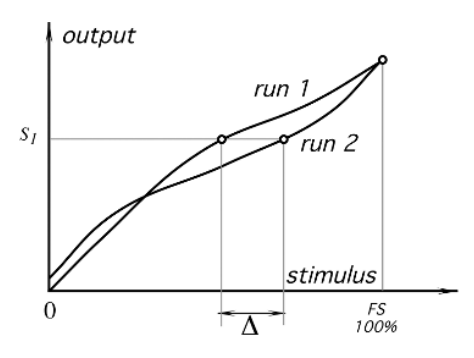
\includegraphics[width=0.9\textwidth]{fig/repeatibility.png}\cite{Fraden_2016}
            \begin{equation*}
                \delta_r = \dfrac{\Delta}{FS}\cdot 100\%
            \end{equation*}
        \end{column}
    \end{columns}
\end{frame}

\begin{frame}{Linealidad y resolución}
    \begin{columns}[c, onlytextwidth]
        \begin{column}{0.55\textwidth}
            \begin{itemize}
                \item Linealidad: es una medida de la proximidad entre la curva de calibración (valores medidos) y una linea recta específica.
                \item Resolución: es el incremento mas pequeño en el valor del estimulo que puede ser medido por el sensor. 
            \end{itemize}
        \end{column}
        \begin{column}{0.40\textwidth}
            \textbf{Ejemplo}\\[4pt]
            Marca: PIHER\\[4pt]
            Modelo: PS2P-LIN\\[4pt]
            Estímulo: posición\\[4pt]
            Tipo: magnetico, efecto Hall\\[4pt]
            Rango del estímulo: $\SI{12}{\milli\meter}$\\[4pt]
            Salida a escala completa (PWM): $10\% (\SI{-6}{\milli\meter}) \sim 90\% (\SI{6}{\milli\meter})$\\[4pt]
            Linealidad: $\pm 1 \%$ \\[4pt]
            Resolución(PWM): $14\,\mathrm{bits}$\\[10pt]
            \tiny{Tomado de \href{https://www.piher.net/pdf/PS2P-LINIntroduction.pdf}{aquí}}
        \end{column}
    \end{columns}
\end{frame}


\begin{frame}{Sensibilidad, saturación y banda muerta}
    \begin{columns}[c, onlytextwidth]
        \begin{column}{0.60\textwidth}
            \begin{itemize}
                \item Sensibilidad: es la pendiente de la curva de calibración, sin importar si es constante o no en todo el rango de salida.  
                \item Saturación: es el rango de operación en el que un incremento en el valor del estímulo no produce variaciones en la señal de salida del sensor. 
                \item Banda muerta: es el rango de operación en el que, sin importar el valor del estímulo, la salida es cercana a cero.
            \end{itemize}
        \end{column}
        \begin{column}{0.35\textwidth}
            \textbf{Ejemplo}\\[4pt]
            Marca: Allegro\\[4pt]
            Modelo: ACS723\\[4pt]
            Estímulo: corriente eléctrica\\[4pt]
            Tipo: magnetico, efecto Hall\\[4pt]
            Rango del estímulo: $\SI{10}{\ampere}$\\[4pt]
            Salida a escala completa: $\SI{0.5}{\volt}(\SI{-5}{\ampere}) \sim \SI{4.5}{\volt}(\SI{5}{\ampere})$\\[4pt]
            Sensibilidad: $\SI{400}{\milli\volt/\ampere}$ \\[4pt]
            Saturación: $<\SI{0.5}{\volt}, >\SI{4.5}{\volt}$\\[10pt]
            \tiny{Tomado de \href{https://www.allegromicro.com/-/media/files/datasheets/acs723-datasheet.ashx}{aquí}}
        \end{column}
    \end{columns}
\end{frame}

\begin{frame}{Valor real, error absoluto y relativo}
    \begin{columns}[c, onlytextwidth]
        \begin{column}{0.55\textwidth}
            \begin{itemize}
                \item Valor real: es el valor de salida que se obtendría con una medición perfecta. Debido a que esto es imposible de determinar se utiliza una convención para definir el valor real.  
                \item Error absoluto: es la diferencia entre una medición y el valor real. 
                \item Error relativo: es el cociente entre el error absoluto y el valor real
            \end{itemize}
        \end{column}
        \begin{column}{0.40\textwidth}
            \begin{equation*}
                \mathrm{error\,absoluto} = \mathrm{medición} - \mathrm{valor\,real}
            \end{equation*}
            \begin{equation*}
                \mathrm{error\,relativo} = \dfrac{\mathrm{error\,absoluto}}{\mathrm{valor\,real}}
            \end{equation*}
        \end{column}
    \end{columns}
\end{frame}

\begin{frame}{Referencias}
\bibliographystyle{ieeetr}
\footnotesize
\bibliography{comunes/referencias}
\end{frame}

\end{document}